\chapter{Pythia - An event exploration web application}\label{Pythia}
\ifpdf
    \graphicspath{{Chapter5/Chapter5Figs/PNG/}{Chapter5/Chapter5Figs/PDF/}{Chapter5/Chapter5Figs/}}
\else
    \graphicspath{{Chapter5/Chapter5Figs/EPS/}{Chapter5/Chapter5Figs/}}
\fi

\section{Pythia - An event exploration web application}\label{WebApp}
Our work in the previous chapters has led to the development of a proof-of-concept web application which can be used to extract and explore
events from Twitter. Pythia can be thought as the last module in the system overview in Figure \ref{SystemOverview}. It provides a graphical user interface that helps humans visualise the results of event detection and summarisation. The main motivation behind the development of this application is to demonstrate the capabilities of our work by looking at historical Twitter data from the Egypt uprising.\\\\
In the next section we describe how the application is built and how it can be used and the rest of the chapter shows the output of Pythia from Egypt's dataset.    

\subsection{Pythia's architecture and design}
The two core components of Pythia is the back-end side which is the data mining system that detects and summarises the events and the front-end side which is the graphical user interface responsible for accepting the user input and visualising the results. Pythia's back-end is built using a scalable, non-blocking web server called Tornado \footnote{http://www.tornadoweb.org/}. This web server is responsible for handling all the request from the front-end and returning the results back. Figure \ref{PythiaOverview} illustrates a very simple diagram of the application. First the front-end receives the user input which is a list of keywords describing the topic the user wants to explore. The list of keywords is passed to the back-end via a HTTP request and a handler is responsible to serve the request. It sends the list of keywords to a data processing module which is nothing more than our event detection system. Our system retrieves the relevant tweets from the database and performs event detection and summarisation. The results are passed by the handler back to the Pythia client and are presented to the user. 

\begin{figure}[htbp]
  \begin{center}
    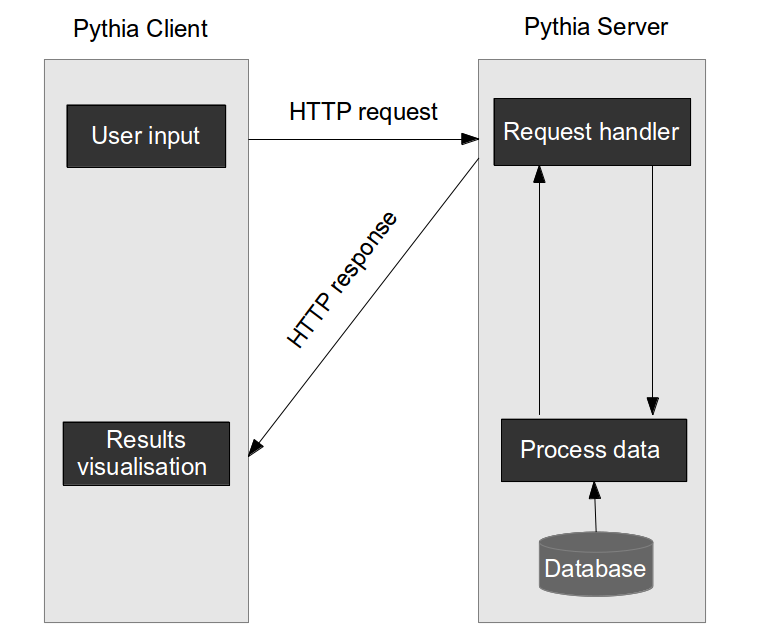
\includegraphics[height=5in, width=6in]{pythia-overview}
    \caption{An overview of Pythia's client-server architecture.}
    \label{PythiaOverview}
  \end{center}
\end{figure} 

\subsection{The Graphical User Interface (GUI) of Pythia}
The motivation behind Pythia is that we wanted to make it as simple as possible for a human to explore and understand events from a Twitter dataset. Therefore, throughout  
the development of Pythia our main consideration was to keep the GUI as lean and simple as possible. The simplicity should not come at the expense of information consumption therefore
another consideration was to give to the user as much information as possible.\\\\
When a user launches Pythia the first page that appears is the one shown in Figure \ref{Pythia1}. A simple text box is used receive the list of keywords provided by the user. The keywords are used to retrieve tweets that contain these words.\\\\
\begin{figure}[htbp]
  \begin{center}
    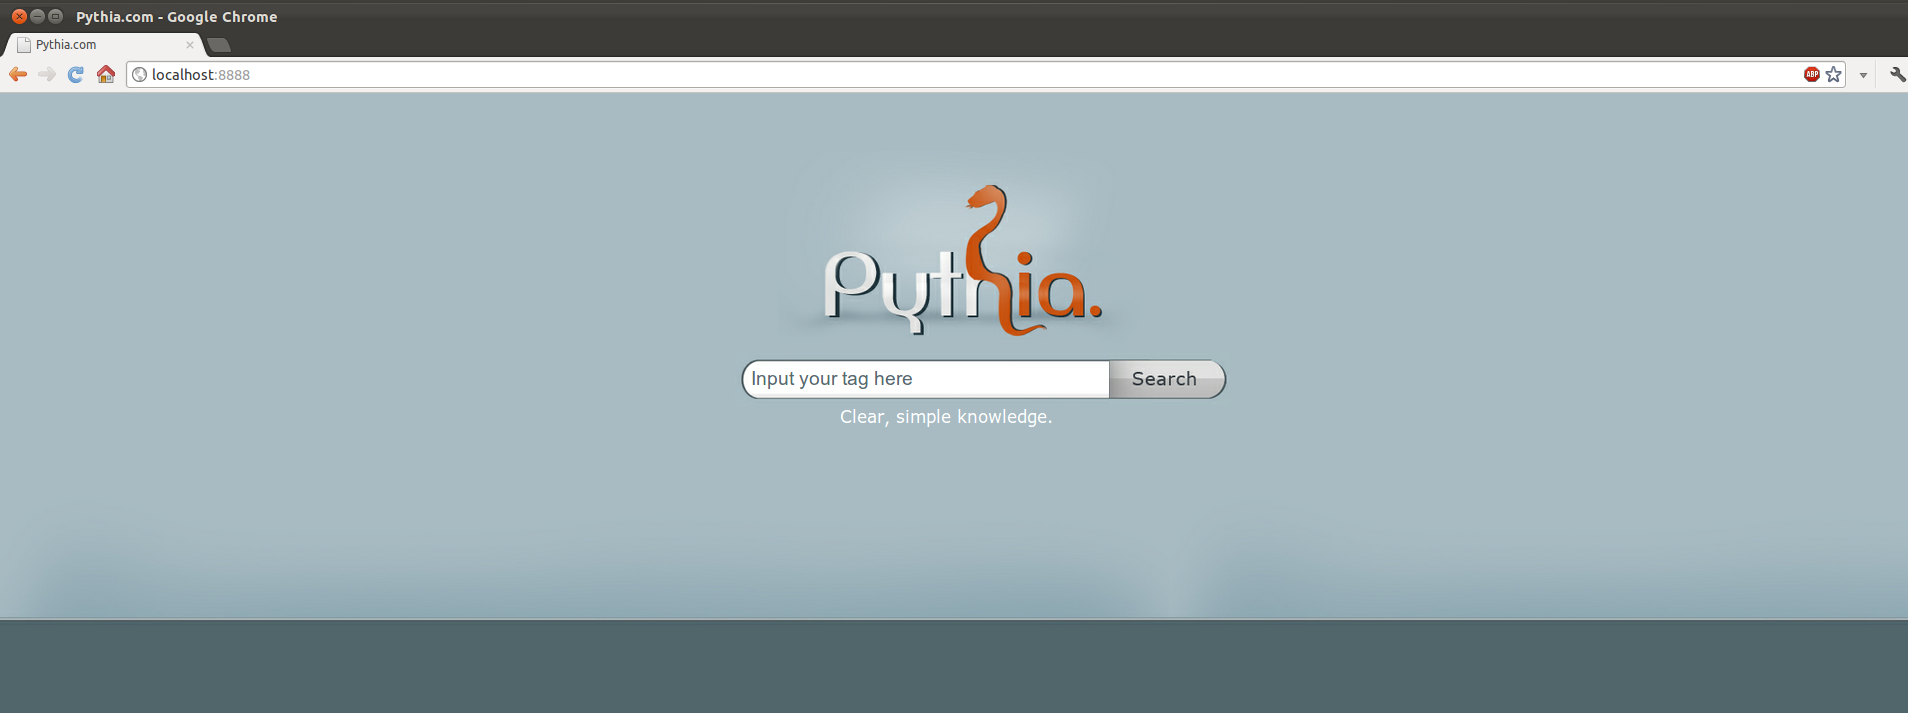
\includegraphics[height=3in, width=6in]{pythia1}
    \caption{The homepage of Pythia. The user inputs in the textbox the keywords related to the events they wish to detect.}
    \label{Pythia1}
  \end{center}
\end{figure} 
The list of keywords is send to the server and the relevan tweets are retrieved from the database. The event detection and summarisation module runs and produces the results which are send back to the user. The detected events appear as small dots on a timeline (Figure \ref{Pythia2}). The x-axis represents time and the y-axis the volume of the tweets in the dataset at that point in time. The smaller timeline on the bottom of the page is a replica of the big one and allows the user to specify a specific time period to zoom in. The timeline allows the user to see the general trend of the events and when they have occured.\\\\    
\begin{figure}[htbp]
  \begin{center}
    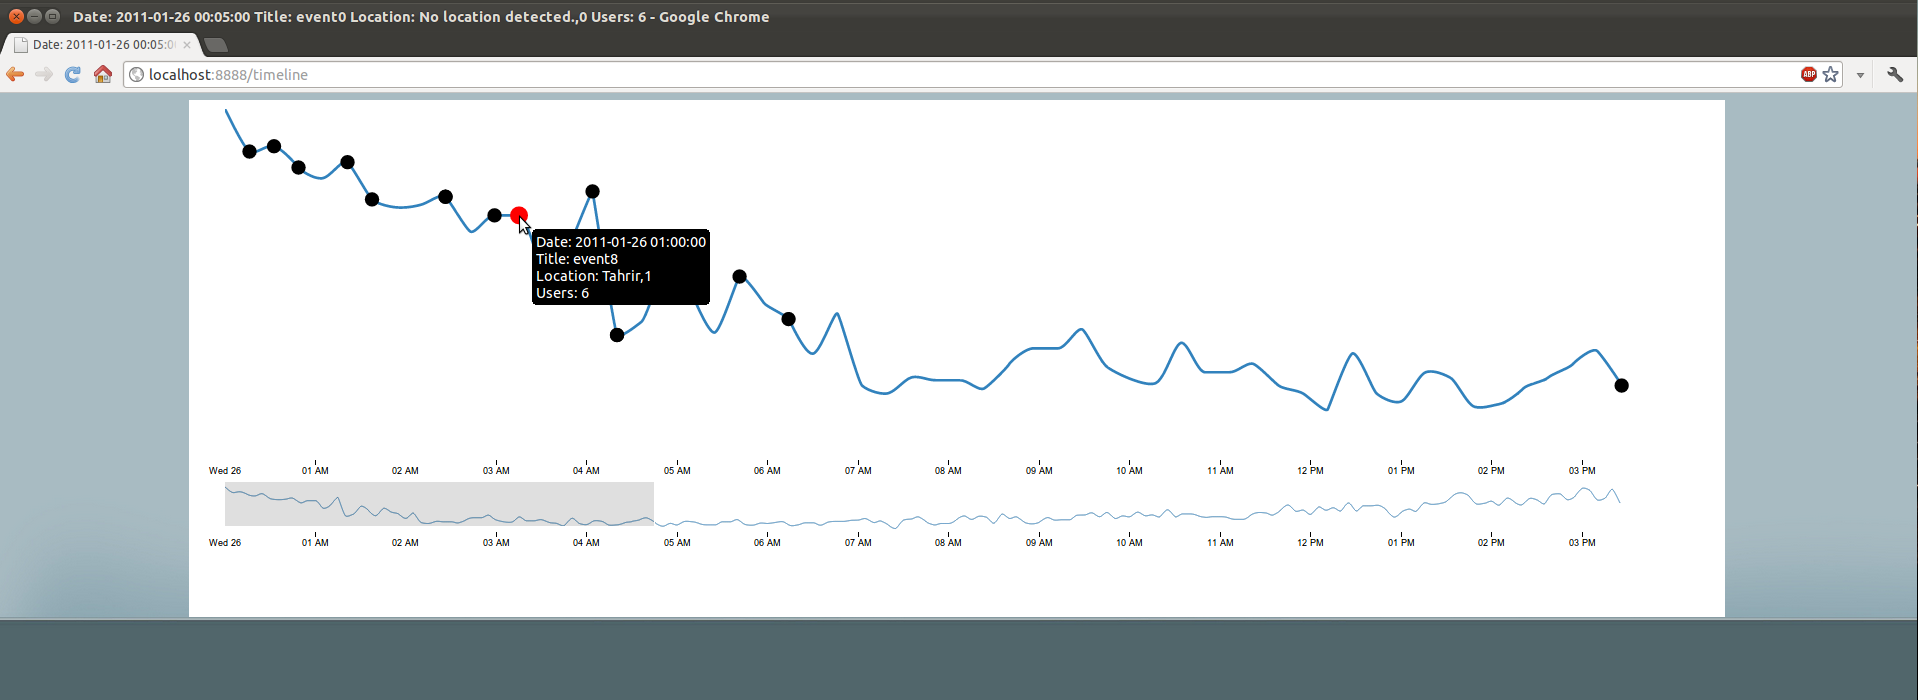
\includegraphics[height=3in, width=6in]{pythia2}
    \caption{The results are presented to the user in the form of an annotated timeline. Each dot on the timeline corresponds to a detected event. The smaller timeline at the bottom of the page allows the    user to zoom in to specific time periods.}
    \label{Pythia2}
  \end{center}
\end{figure} 
In order to understand the events more information is needed. Therefore, we have created a special popup window which displays the results of the summarisation algorithm in a human readable way. This popup window is shown in Figure \ref{Pythia3}. The user can clearly see which tweets have the highest ranking according to the LexRank algorithm and the top keywords related to the event. Additionally, if any named-entities or locations have been identified they are displayed in the relevant sections. Finally, the pie chart in the right hand corner demonstrates the results of the user classification module by showing the proportions of the user types occuring in this event.    
\begin{figure}[htbp]
  \begin{center}
    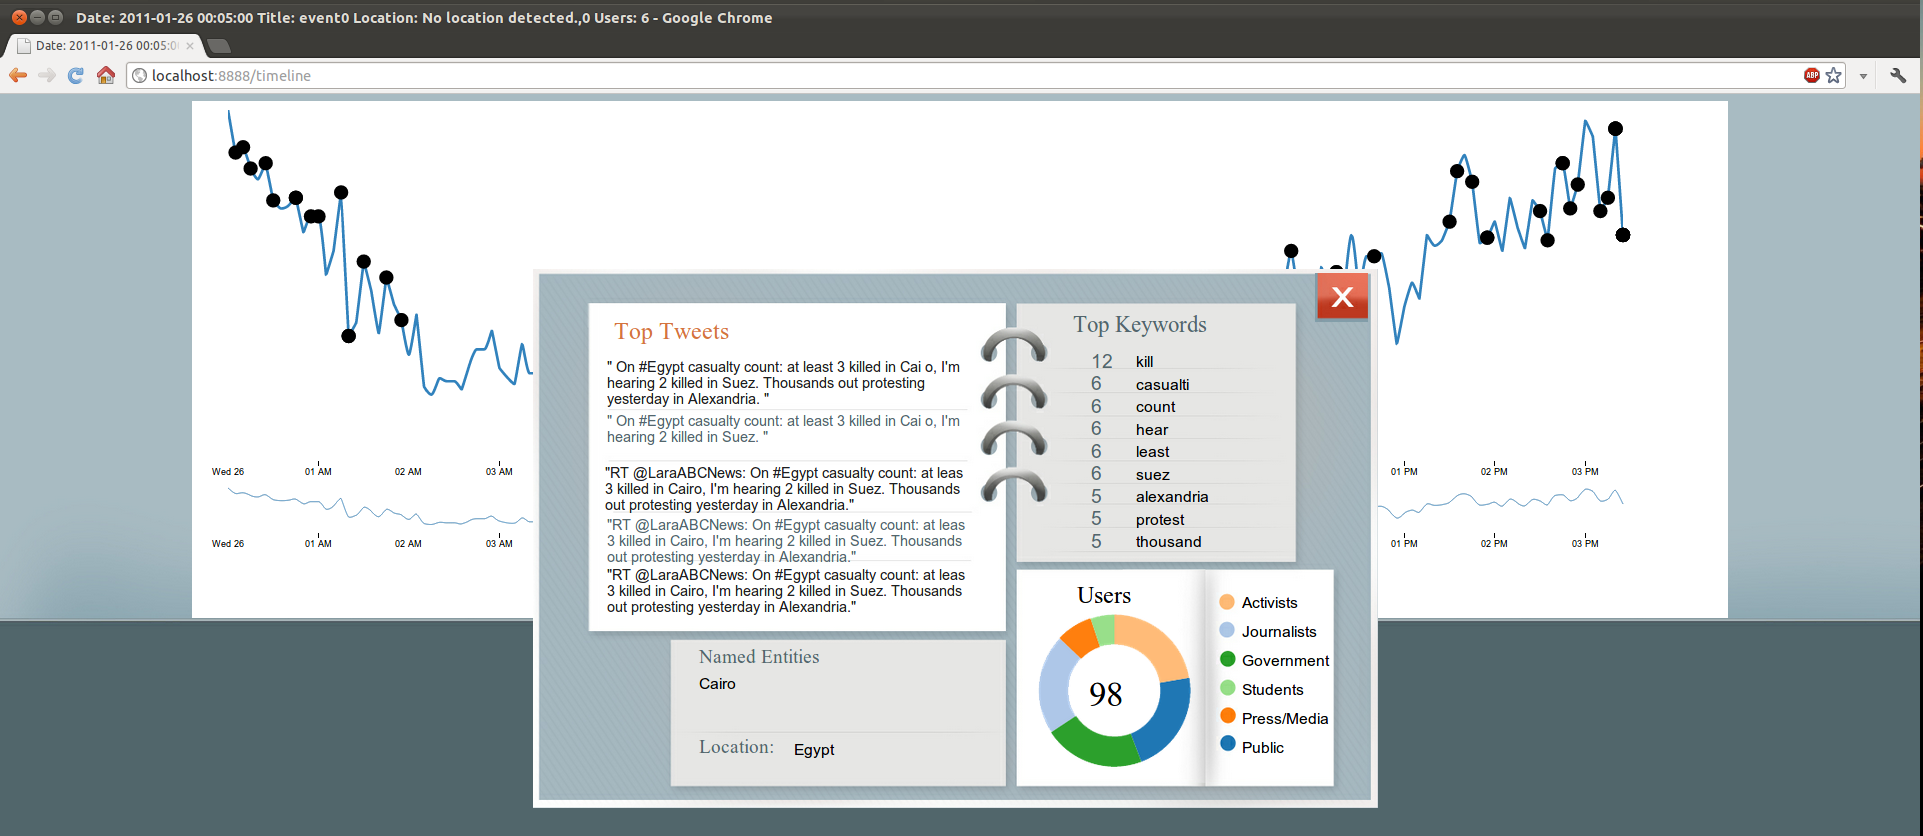
\includegraphics[height=3in, width=6in]{pythia3}
    \caption{The event summary popup helps the user understand what an event is about.}
    \label{Pythia3}
  \end{center}
\end{figure} 

\section{Case study on a clean dataset}
\subsection{Results and discussion}

\section{Case study on a real dataset}
\subsection{Results and discussion}

\section{Summary}

% ------------------------------------------------------------------------


%%% Local Variables: 
%%% mode: latex
%%% TeX-master: "../thesis"
%%% End: 
